\section{Análisis estructural}\label{sec:fea}

El diseño de este prototipo fue ampliamente debatido. Para llegar a buen puerto con las decisiones de ingeniería, lo que se utilizó fue la herramienta de elementos finitos. Más allá del buen planteo del diseño inicial, necesario para poder optimizar luego el prototipo. Si se plantea de manera errónea el problema, no se justifica una optimización estructural, es por ello que desde el comienzo con el diseño preliminar se itero para poder obtener un diseño acorde, para luego ser optimizado. Un diseño erroneo inicial, no hay elemento finito que lo arregle. Por esto fue crucial en base a la experiencia adquirida en estos años de estudios, proyectos personales poder
plantear un diseño inicial bien encaminado hacia los requerimientos para poder soportarlas necesidades en las condiciones de prueba. Se necesita obtener un coeficiente de peso y resistencia que sea apropiado para poder probar el sistema de control en el vehículo, logrando que vuele y que aterrice, pudiendo volver a realizar la maniobra en condiciones nominales. Estos procedimientos consisten en realizar con el vehículo parado por sus propios medios, un despegue y un aterrizaje de manera autónoma, controlando mediante software. De esta manera poder llegar a la finalización del proyecto en condiciones mecánicas funcionales, es decir, poder modificar de manera correcta el sistema de control sin destrozar el prototipo en el camino. 

\medskip

Para poder lograr el objetivo de probar un sistema de control en un vehículo autónomo de características VTVL, se necesita que el fuselaje tenga los siguientes requerimientos:

\begin{itemize}
    \item Que no se desarme ninguna parte en un aterrizaje en condiciones nominales. 
    \item Que ante una caída luego del aterrizaje, de lado, no se pierda funcionalidad del vehículo.
    \item Que sea capaz de llevar 1kg de payload, además del peso propio.
    \item Que la electrónica se pueda anclar mecánicamente y ser integrada dentro de él.
    \item Que los cables pasen por el interior del vehículo.
    \item Que se le puedan realizar reformas de ubicación de componentes, por posibles complicaciones en el futuro con los componentes.
    \item Que se pueda armar en las instalaciones de LIA Aerospace.
    \item Debe ser replicable ante un hecho que destruya el vehículo y deba ser rearmado desde el comienzo.
    \item Que las cargas del EDF y del aterrizaje puedan ser soportadas, con un factor de seguridad mayor a 1,4 ante la plastificacion. (REFERENCIA)
    \item Que no tenga daños por corrosión en la duración del proyecto.
    \item Que permita ser construido con materiales disponibles en la región.
    \item Que no interrumpa el paso del flujo de aire al EDF.
    \item Que se pueda armar con herramientas disponibles en un taller con herramientas manuales, torno y fresa. 
    \item Que no se involucre una maquina CNC por los costos asociados al proyecto, los tiempos y el contexto pandemia por tercerización.
    \item Disposición de masas semejante a un cohete esbelto.
    \item Que su geometría permita puntos de anclajes para poder realizar las pruebas.
    \item Que permita modificaciones por secciones, para poder acceder a la electrónica.
    \item Que permita que el flujo saliente del EDF pueda ser controlado y tenga una via de escape que no interfiera con otros componentes.
    \item Capacidad de anexar flaps inferiores para control de rolido.
    \item Alojamiento de servos para giros de gimball.
    \item Capacidad de alojar un elemento de suspensión.
    \item Que el vehículo se quede parado.
    \item Que quede balanceado en un plano paralelo al rotor del EDF.
\end{itemize}

\medskip

El fuselaje fue la parte mecánica con mayor cantidad de iteraciones, se pasó por distintos prototipos. Cada uno de ellos fue pensado en el diseño intentando llevar a su geometría a la forma más eficiente teniendo en consideración los flujos de aire, las cargas y el peso, intentando desde el diseño preliminar en lápiz y papel favorecer a un bajo peso para una resistencia adecuada del componente. Para la condición de vuelo, las cargas eran el empuje del EDF y el peso principalmente, al estar en un caso de baja aceleración en los objetivos del proyecto, para este caso se encontró que las limitaciones eran las geométricas. 

Se continuó con el modelado de la estructura imponiéndole una fuerza en la parte superior y como parámetro de decisión se utilizó el criterio que suele utilizarse en el ámbito aeroespacial que es ponerle a distintas estructuras 1 N de fuerza y ver entre ellas cuál es la más eficiente para este caso de carga. Para luego decidir entre estos prototipos analizando los casos de tensiones máximas entregadas por el modelado del elemento finito. La razón por la cual se usa un caso de carga de 1N es para además rápidamente estimar la fuerza a la cual entra en fluencia para el caso de un modelo lineal. La cuenta para lograr esto es dividendo la tensión de fluencia del material por la tensión máxima en el modelo se obtiene la fuerza necesaria para que el punto entre en fluencia.

Se detectó que el aterrizaje era la peor condición, así que se diseñó y modeló para este caso. No se estudiara el impacto al desconocer los factores dinámicos. Siendo el peor escenario posible caer con solo una pata a impacto y de costado, pero en el segundo rebote, es decir tocar el piso a impacto y luego al girar que soporte todo el peso del vehículo sin plastificar de costado, multiplicado por 1,4 que fue el factor de seguridad elegido.  Se decidió corroborar a fluencia la carga lateral mencionada en la pata y en el extremo superior con una carga de 100 N que resulta de multiplicar 7 kilogramos con el factor de seguridad elegido 1,4 en base a \cite{zipay2016ultimate}:

\begin{equation}
    F = 7 kg * 9,81 m/s^2 * 1,4 = 96.138 N \approx 100 N
\end{equation}

En la finalización del proyecto se encontró que esta predicción fue correcta para el peso del vehículo.


Se hicieron varios modelos de distintos prototipos de fuselajes con elementos finitos, varios de estos modelos quedaron a disposición de la empresa LIA Aerospace y no pueden ser mostrados por cuestiones de tratados confidenciales. A continuación se mostraran aquellos que agregan información de cómo se llegó al prototipo final de este modelo en particular.

En total se han planteado 11 conjuntos de CAD distintos con fuselajes distintos para luego ser modelados.


\null\newpage
\clearpage

\subsection{Modelo y simulación propuesta tipo jaula}
En una primera instancia se propuso un diseño tipo jaula. Este diseño tenia varias ventajas con respecto al de acceso a componentes electrónicos, pero tenia una dificultad de armado con respecto a otros prototipos que se estaban planteando, también muchas mas horas de soldadura, se agrandaba axisimétricamente, generando una figura circular a base de caños rectos, haciendo que sea difícil de replicar, balancear y construir.

Se analizo previamente mediante un modelado de elementos finitos para poder contrastar con otros modelos.

Se aplico una carga de 1 N en dirección del plano del rotor del EDF y colineal a una de las patas, con dirección entrante al eje de axsimetría, aplicado en la parte superior del fuselaje, con las patas empotradas en donde hacen contacto al suelo.

Se puede ver en la siguiente imagen el resultado de la simulación de elementos finitos, para el caso de desplazamientos nodales.


\begin{figure}[htb]
    \centering
    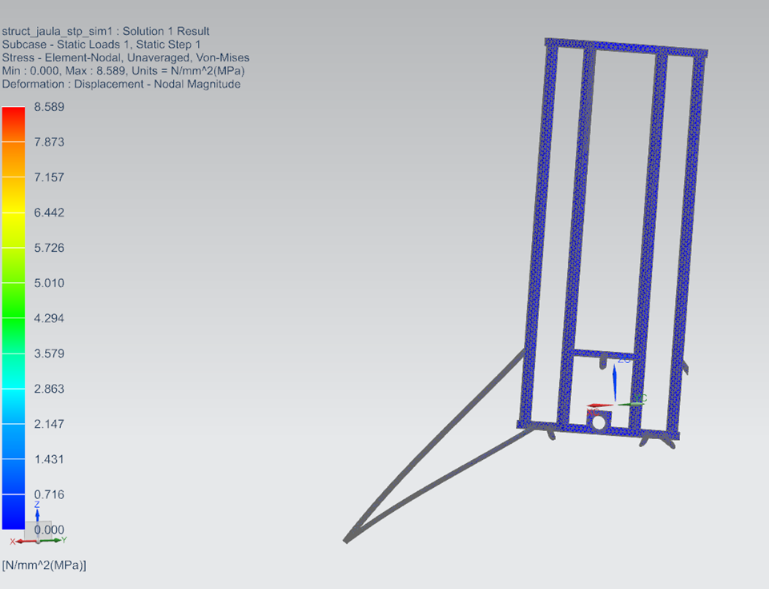
\includegraphics[height=0.4\pdfpageheight]{fig/fea/jaula.png}
    \caption{Modelado inicial estructura esfuerzos para carga de 1N estático en las patas dirección normal al suelo modelo de fuselaje tipo jaula.}
    \label{fig:fea/jaula}
\end{figure}

A continuación se muestra el detalle del corte para el mismo caso, análisis de tensiones.

Se puede apreciar que se estaba en una coloración verde, medianamente solicitado, en la parte de las patas mas comprometida, y el resto de la estructura se encontraba en baja carga, coloración azul.

\begin{figure}[htb]
    \centering
    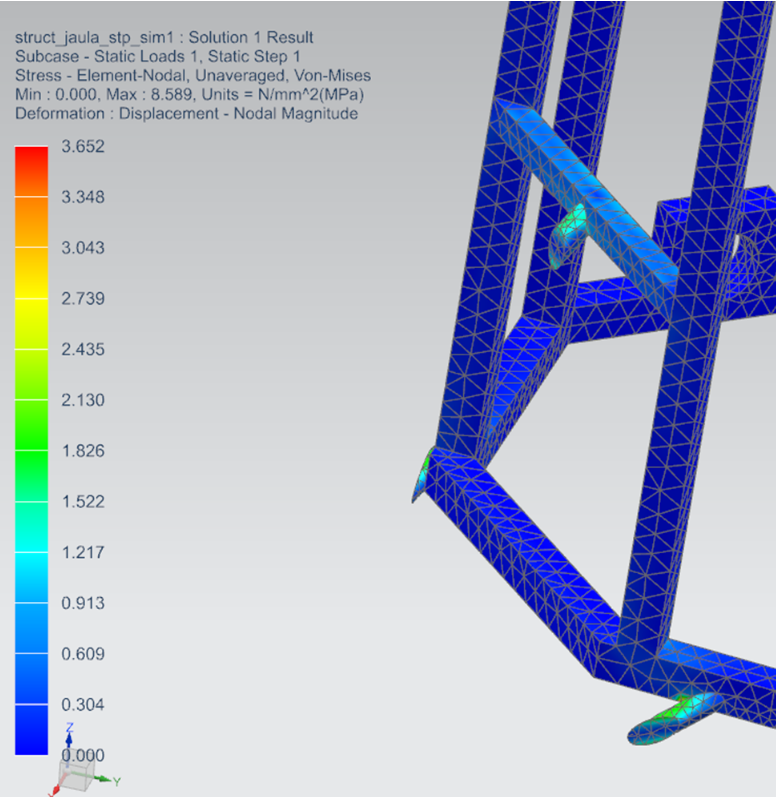
\includegraphics[height=.5\pdfpageheight]{fig/fea/jaula2.png}
    \caption{Esfuerzos para carga de 1N estático para misma condición de la figura anterior, solo vista de esfuerzos de la parte superior quitando las patas.}
    \label{fig:fea/jaula2}
\end{figure}



\null\newpage
\clearpage

\subsection{Modelo y simulación del fuselaje tubo y placas vaciadas}

Se propuso un prototipo diferente, que se comenzó a iterar. Consiste en un tubo y un aro, soldado a 4 placas que conforman las patas. Se comenzó quitando material al centro de las placas vaciadas que son las patas y se procedió a simular para 1 N en dirección del plano del rotor del EDF y colineal a una de las patas, con dirección entrante al eje de axisimetría, aplicado en la parte superior del fuselaje, con las patas empotradas por donde hacen contacto al suelo. Para poder comparar su comportamiento frente a otros prototipos.

A continuación se muestra una vista de las tensiones en la figura \ref{fig:fea/tuboplaca1} y los desplazamientos en la figura \ref{fig:fea/tuboplaca2} para este caso.

Se puede extrapolar que para una carga de 100N se tiene una tensión de 16MPa,\footnote{Se aplicaban cargas de 1N y seobtuvo 0.16MPa de tensión máxima. Para obtener la tensión máxima a 100N se puede multiplicar 0.16 por 100 ya que se aplica la teoría de elasticidad lineal.} que se esta fuera de la fluencia con un factor de seguridad mayor a 17 (276 MPa a fluencia) en el punto mas solicitado, siendo aun mayor en puntos de interés, como en los espesores de los brazos conformados por el vaciado de las patas. También que los desplazamientos se encuentran en un valor bajo, siendo el mayor valor 0.5 mm. Con lo cual se procedió a seguir quitando material del fuselaje realizando otros vaciados.

Se simulo la deflexión en una pata lateral. Resultado de una posible caída con el peso del vehículo. Se impuso una carga de 100N lateral,  (resultado de multiplicar el peso estimado del vehículo por 1.4 y la gravedad). En el peor caso para esa condición, es decir la fuerza ortogonal a la placa en el extremo mas alejado. Como condición de borde se anclaron las demás patas.

En la figura \ref{fig:fea/tuboplaca4} se muestra el resultado para los desplazamientos aplicando 100 N en una de sus patas. Se puede observar que los desplazamientos no son significativamente grandes. Y por último para esta condición se muestra el resultado para las tensiones aplicando 100 N en una de sus patas mostrados en la figura \ref{fig:fea/tuboplaca5}.

Se puede observar que las tensiones están con un factor de seguridad de 2, estando por debajo de las tensiones máximas para el punto más solicitado.

Por último se muestran las masas e inercias del fuselaje analizado en la figura \ref{fig:fea/tuboplacainercias}.

\begin{figure}[htb]
    \centering
    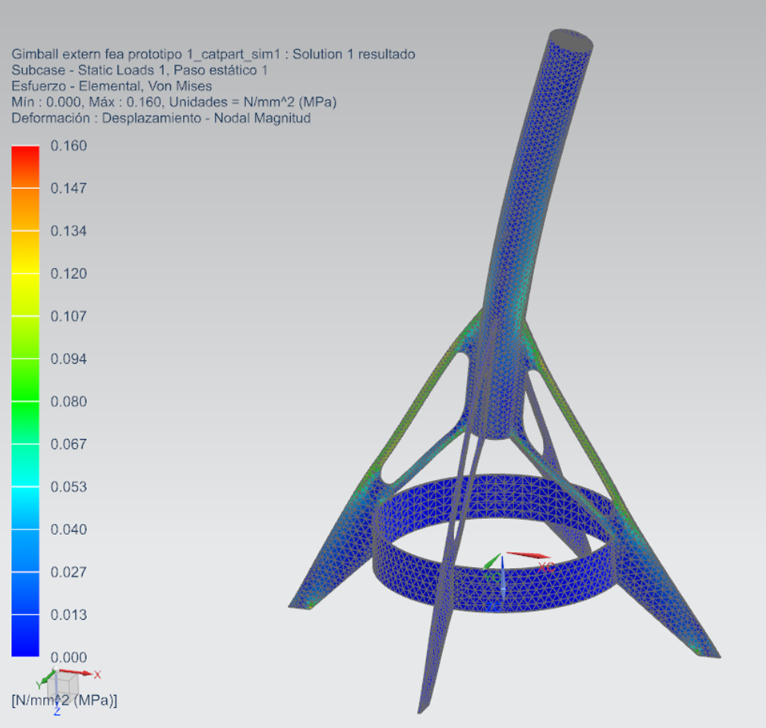
\includegraphics[height=0.27\pdfpageheight]{fig/fea/tuboplaca1.png}
    \caption{Modelo tubo y placas esfuerzo elemental para carga superior de 1 N en dirección planar al suelo.}
    \label{fig:fea/tuboplaca1}
\end{figure}

\begin{figure}[htb]
    \centering
    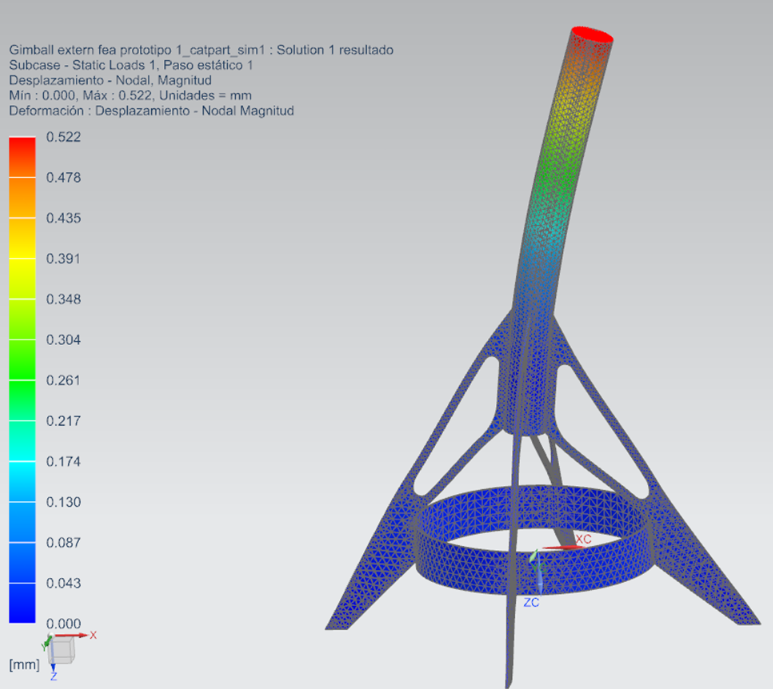
\includegraphics[height=0.27\pdfpageheight]{fig/fea/tuboplaca2.png}
    \caption{Modelo tubo y placas desplazamiento elemental para carga superior de 100 N en dirección planar al suelo.}
    \label{fig:fea/tuboplaca2}
\end{figure}


\begin{figure}[htb]
    \centering
    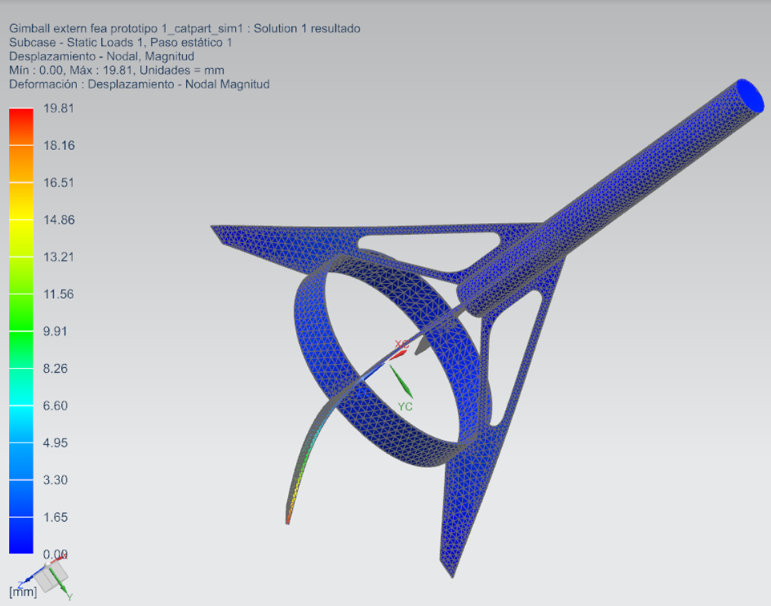
\includegraphics[height=0.3\pdfpageheight]{fig/fea/tuboplaca4.png}
    \caption{Modelo tubo y placas deformación en una de sus patas con una carga de 100N en dirección normal a la superficie de una de sus patas.}
    \label{fig:fea/tuboplaca4}
\end{figure}

\begin{figure}[htb]
    \centering
    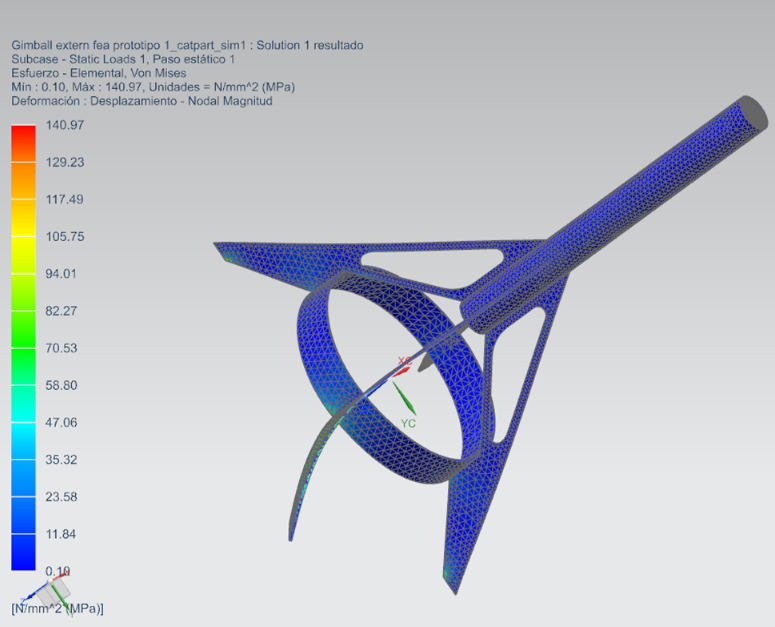
\includegraphics[height=0.3\pdfpageheight]{fig/fea/tuboplaca5.png}
    \caption{Modelo tubo y placas esfuerzo en una de sus patas con una carga de 100N en dirección normal a la superficie de una de sus patas.}
    \label{fig:fea/tuboplaca5}
\end{figure}


\begin{figure}[htb]
    \centering
    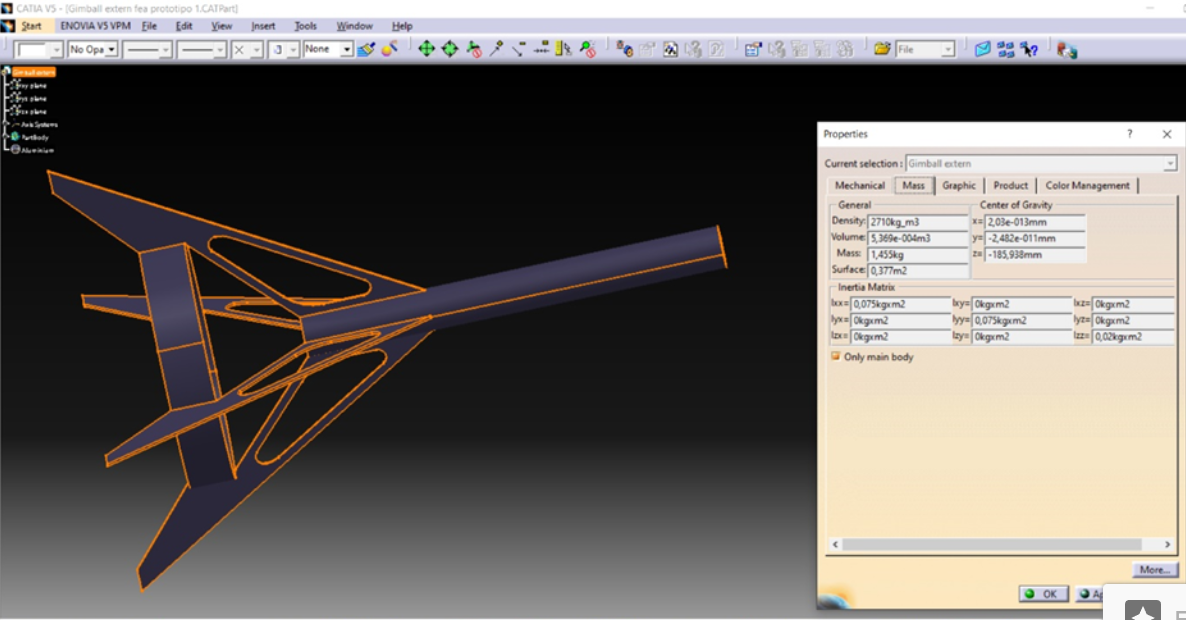
\includegraphics[height=0.27\pdfpageheight]{fig/fea/inercias}
    \caption{Peso e inercias del prototipo analizado.}
    \label{fig:fea/tuboplacainercias}
\end{figure}

\null\newpage
\clearpage

\subsection{Iteración del modelo y simulación en la que se definió la geometría final de las placas que componen las patas}


Se procedió a seguir realizando varios vaciados, iterando de manera de no sobrepasar las tensiones máximas y estar en un factor de seguridad cercano a 1.4.

Se decidió remover material del centro del soporte del gimbal. Esto trae como ventaja también la facilidad de rolado de la chapa para el proceso productivo de armar el fuselaje, al tener menor sección resistente al trabajado mecánico en frio.

Se impuso una carga de 1 N en dirección del plano del rotor del EDF y colineal a una de las patas, con dirección entrante al eje de axisimetría, aplicado en la parte superior del fuselaje, con las patas empotradas por donde hacen contacto al suelo.

Resultado de esta condición para desplazamientos en la figura \ref{fig:fea/patas1} y esfuerzos en la figura \ref{fig:fea/patas2}. Se observo un deplazamiento máximo de menos de una centesima de milímetro, y un esfuerzo máximo de 0.27MPa.

El punto mas solicitado se encuentra en una de sus patas donde se preveía que iba a estar, en la parte donde tracciona la sección disminuida por momento flexor.

Se continuo con la idea de modelar la pata vaciada con una carga de 100 N, en la misma condición que la sección 4.2, en la dirección normal a una de sus patas manteniendo las demás ancladas. 

Resultado de esta condición para desplazamientos en la figura \ref{fig:fea/patas3} y esfuerzos en la figura \ref{fig:fea/patas4}. Se puede observar que aun se esta por debajo de los 276 MPa, pero acercándose a factor de seguridad 1.4.

La figura \ref{fig:fea/patas5} contiene datos de masas e inercias.

La figura \ref{fig:fea/imagenpatas} corresponde al conjunto ensamblado que se había propuesto para este prototipo.

\medskip

Se comprobó que las patas aguantaron las cargas de diseño para su peor condición con
factor de seguridad mayor a 1.4.
Como se vio que la estructura tubular estaba sobredimensionada para ser portadora de
los componentes electrónicos, sin más análisis se procedió al vaciado para poder acceder
a la electrónica. Se optó por una cuestión de simplicidad y avance con los tiempos de
manufactura de prescindir del cono invertido, quedando tubular el diseño final del
fuselaje.



\begin{figure}[htb]
    \centering
    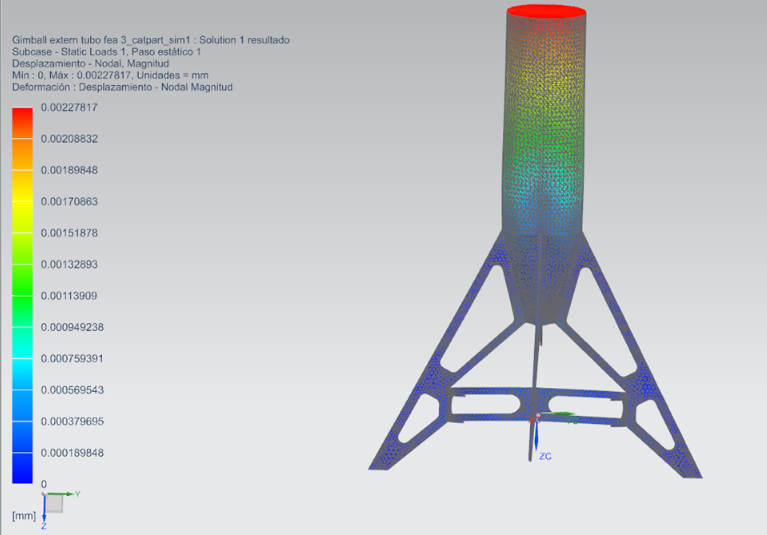
\includegraphics[height=0.2\pdfpageheight]{fig/fea/patas1.png}
    \caption{Modelo tubo y placas iteración $n$ desplazamiento para carga superior 1 N en dirección planar al suelo.}
    \label{fig:fea/patas1}
\end{figure}

\begin{figure}[htb]
    \centering
    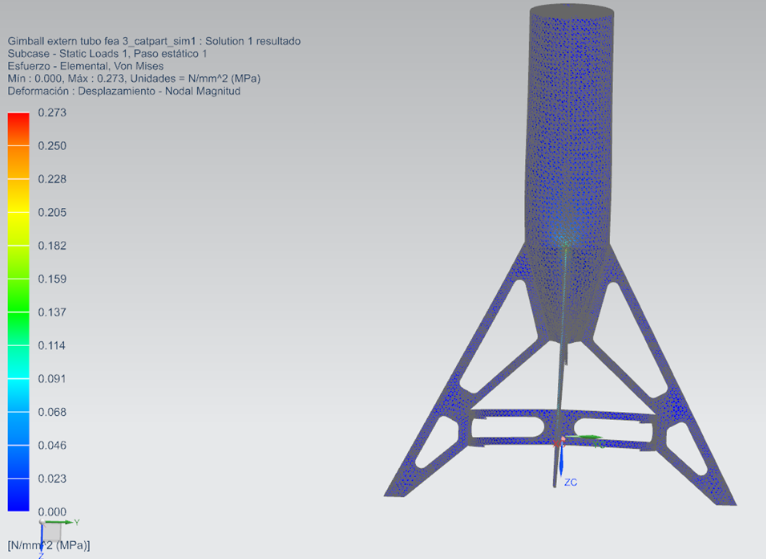
\includegraphics[height=0.25\pdfpageheight]{fig/fea/patas2.png}
    \caption{Modelo tubo y placas iteración $n$ esfuerzos elementales para carga superior 1 N en dirección planar al suelo.}
    \label{fig:fea/patas2}
\end{figure}

\begin{figure}[htb]
    \centering
    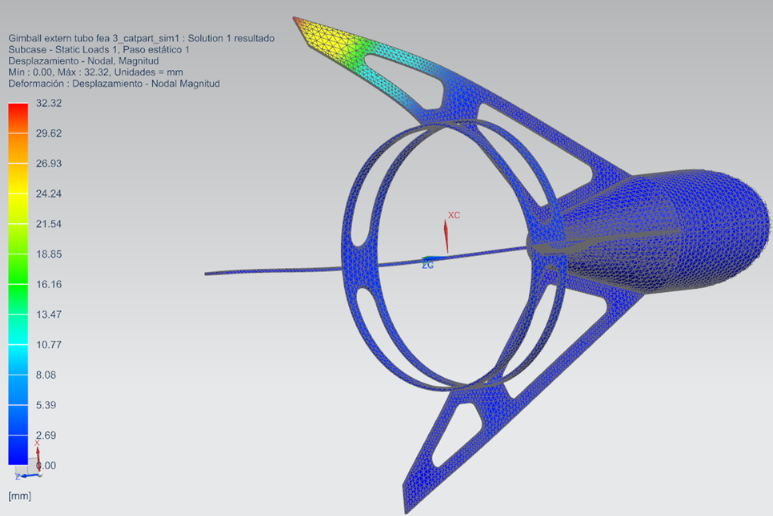
\includegraphics[height=0.3\pdfpageheight]{fig/fea/patas3.png}
    \caption{Modelo tubo y placas iteración $n$ desplazamientos con cargas de 100N en dirección normal a la superficie de una de sus patas.}
    \label{fig:fea/patas3}
\end{figure}


\begin{figure}[htb]
    \centering
    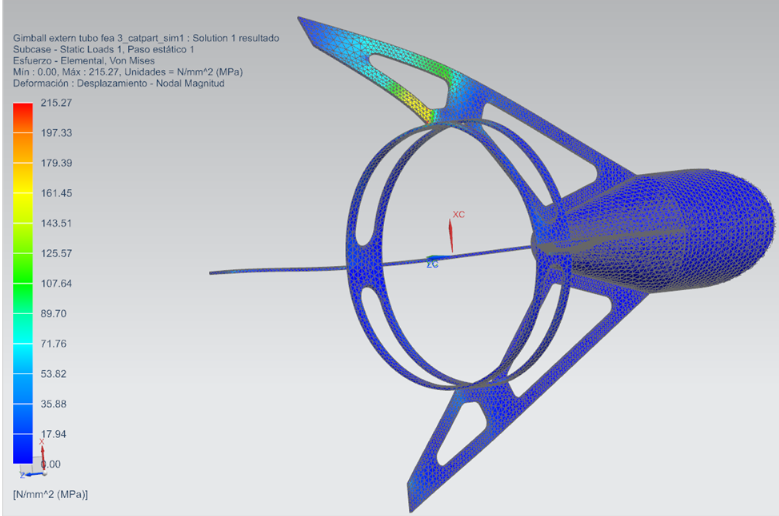
\includegraphics[height=0.3\pdfpageheight]{fig/fea/patas4.png}
    \caption{Modelo tubo y placas iteración $n$ esfuerzos elementales con carga de 100N en dirección normal a la superficie de una de sus patas.}
    \label{fig:fea/patas4}
\end{figure}

\begin{figure}[htb]
    \centering
    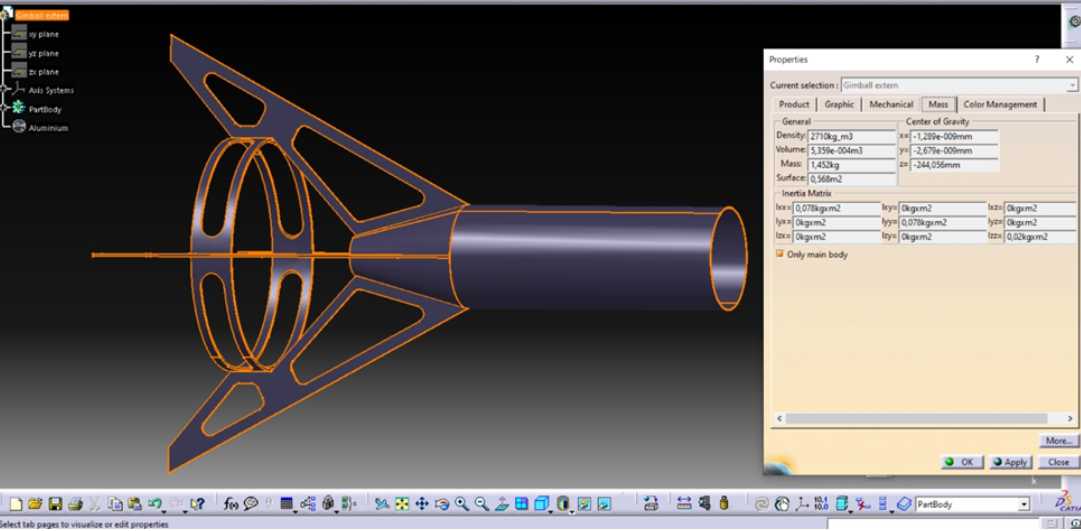
\includegraphics[height=0.25\pdfpageheight]{fig/fea/inerciaspatas.png}
    \caption{Peso e inercias del prototipo analizado.}
    \label{fig:fea/patas5}
\end{figure}

\begin{figure}[htb]
    \centering
    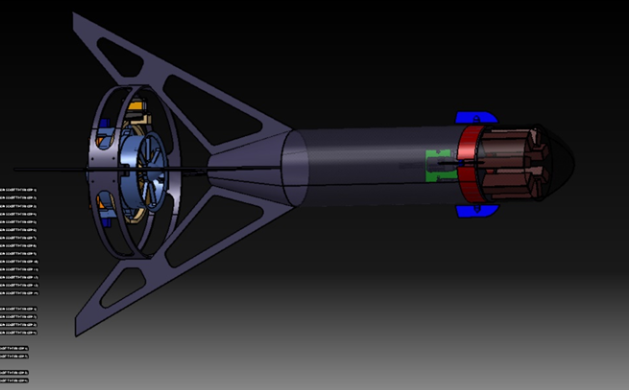
\includegraphics[height=0.3\pdfpageheight]{fig/fea/imagenpatas.png}
    \caption{Imagen del conjunto del prototipo analizado.}
    \label{fig:fea/imagenpatas}
\end{figure}


